\newcommand{\NWtarget}[2]{#2}
\newcommand{\NWlink}[2]{#2}
\newcommand{\NWtxtMacroDefBy}{Fragment defined by}
\newcommand{\NWtxtMacroRefIn}{Fragment referenced in}
\newcommand{\NWtxtMacroNoRef}{Fragment never referenced}
\newcommand{\NWtxtDefBy}{Defined by}
\newcommand{\NWtxtRefIn}{Referenced in}
\newcommand{\NWtxtNoRef}{Not referenced}
\newcommand{\NWtxtFileDefBy}{File defined by}
\newcommand{\NWtxtIdentsUsed}{Uses:}
\newcommand{\NWtxtIdentsNotUsed}{Never used}
\newcommand{\NWtxtIdentsDefed}{Defines:}
\newcommand{\NWsep}{${\diamond}$}
\newcommand{\NWnotglobal}{(not defined globally)}
\newcommand{\NWuseHyperlinks}{}
\documentclass[a4paper]{report}
\newif\ifshowcode
\showcodetrue
\usepackage{cite}
\usepackage{latexsym}
%\usepackage{html}
\usepackage{lscape}
\usepackage{listings}
\usepackage{graphicx}
\usepackage{color}
\definecolor{linkcolor}{rgb}{0, 0, 0.7}

\usepackage[%
backref,%
raiselinks,%
pdfhighlight=/O,%
pagebackref,%
hyperfigures,%
breaklinks,%
colorlinks,%
pdfpagemode=None,%
pdfstartview=FitBH,%
linkcolor={linkcolor},%
anchorcolor={linkcolor},%
citecolor={linkcolor},%
filecolor={linkcolor},%
menucolor={linkcolor},%
pagecolor={linkcolor},%
urlcolor={linkcolor}%
]{hyperref}

\setlength{\oddsidemargin}{0in}
\setlength{\evensidemargin}{0in}
\setlength{\topmargin}{0in}
\addtolength{\topmargin}{-\headheight}
\addtolength{\topmargin}{-\headsep}
\setlength{\textheight}{8.9in}
\setlength{\textwidth}{6.5in}
\setlength{\marginparwidth}{0.5in}

\title{GML-DOT 1.0 \\ A Graph Translation Tool}
\date{}
\author{Philip Gabardo}
\pagenumbering{roman}

\begin{document}
\maketitle
\tableofcontents

\chapter{Introduction}
\section{Summary}
The proposed project is a compiler that translates graphs represented in Graph Modelling Language (GML) to a visual PDF representation produced through DOT code.

 GML \cite{GML}is a file format standard that is used for representing graphs. GML's key features are portability, simplicity, extensibility and flexibility. The syntax consists of hierarchical key-value lists. Here is an example of a very simple GML file:
 \begin{verbatim}
graph [
	comment "This is a sample graph"
	directed 1
	id n42
	label "Hello, I am a graph"
	node [
		id 1
		label "node 1"
	]
	node [
		id 2
		label "node 2"
	]
	node [
		id 3
		label "node 3"
	]
	edge [
		source 1
		target 2
		label "Edge from node 1 to node 2"
	]
	edge [
		source 2
		target 3
		label "Edge from node 2 to node 3"
	]
	edge [
		source 3
		target 1
		label "Edge from node 3 to node 1"
	]
]
\end{verbatim}

There are several other languages that closely resemble GML, such as GDF\cite{GDF}, GraphML\cite{GRAPHML}, and DOT\cite{DOT}.

GML is widely used, and is the standard file format in the Graphlet graph editor system.

A major drawback of GML is its lack of direct graph translation to png or pdf images, which is essential to users would who like to visualize their graphs. Consequently, many users choose languages such as DOT, which can produce png and pdf images to represent their graphs, despite GML's attempt to become a universal file format for graphs.

 The purpose of this compiler is to give GML users the ability to visualize their graphs through translation to DOT code, which can be used to generate a nicely formatted png file. DOT syntax is very simple, and contains single line statements to declare nodes and edges. The compiler will provide a simple, structure-preserving translation. Here is an example of the DOT code and the visual representation (generated using the DOT code) of the graph described in the sample GML provided earlier:
\begin{verbatim}
graph G {
	label = "My graph";
	comment = "This is a test";
	1 [label = "Node 1"];
	2 [label = "Node 2"];
	3 [label = "Node 3"];
	4 [label = "test"];
	1 -- 2 [label = "Edge from node 1 to node 2"];
	2 -- 3 [label = "Edge from node 2 to node 3"];
	3 -- 1 [label = "Edge from node 3 to node 1"];
}

\end{verbatim} 


 \begin{center}
 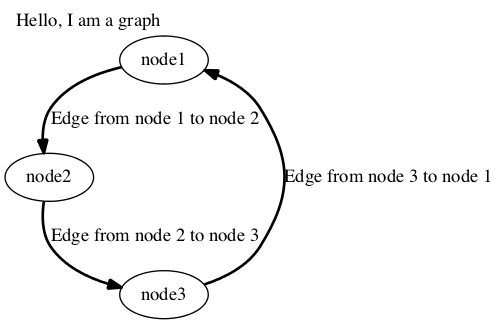
\includegraphics[scale=0.5]{test}
 \end{center}
 
\section{Tools}
The following tools were used for this project:
\begin{itemize}
\item \textbf{ANTLR4}\cite{ANTLR4} was be used to generate DOT code from given GML code. ANTLR4 was chosen for two main reasons. First, ANTLR4 is proven to produce correct grammars. The generated parser accepts exactly the language specified in the grammar. If a recursive descent parser was used instead, there would be no immediate proof of correctness, and no easy way to test it. Secondly, ANTLR4 was chosen for its speedy development time. The parser and lexer rules can be constructed extremely fast.
\item \textbf{DOT}\cite{DOT} was used to draw the graphs. DOT was chosen because it is can automatically place nodes and edges such that there is minimal overlap (developing this kind of algorithm is outside the scope of this course). Furthermore, DOT has a command-line tool for producing png and pdf files, which many other graph languages that have automatic placement lack. For example, yWorks\cite{YWORKS} requires the user to import their graphs to an editor in order to view them.
\item \textbf{nuweb}\cite{NUWEB} was be used to document the project. nuweb was chosen because it supports any programming language (there are no literate programming tools specificly targetted for ANTLR), it is documented well, and it has plenty of user support through forums. nuweb was chosen over noweb because noweb is heavily Unix-dependent, and requires many third party programs in order to be built.
\end{itemize}

\chapter{Implementation}
The high-level flow of steps for the compiler is as follows:
\begin{enumerate}
\item Parse the GML file to elicit an object based representation of the graphs.
\item Convert the object based representation of the graphs to DOT.
\end{enumerate}

The ANTLR compiler is organized as follows: 
\begin{flushleft} \small
\begin{minipage}{\linewidth}\label{scrap1}\raggedright\small
\NWtarget{nuweb1}{} \verb@"GMLDot.g4"@\nobreak\ {\footnotesize {1}}$\equiv$
\vspace{-1ex}
\begin{list}{}{} \item
\mbox{}\verb@@\\
\mbox{}\verb@@\hbox{$\langle\,${\itshape Grammar Name}\nobreak\ {\footnotesize \NWlink{nuweb12}{12}}$\,\rangle$}\verb@@\\
\mbox{}\verb@@\hbox{$\langle\,${\itshape Header}\nobreak\ {\footnotesize \NWlink{nuweb2}{2}}$\,\rangle$}\verb@@\\
\mbox{}\verb@@\hbox{$\langle\,${\itshape Members}\nobreak\ {\footnotesize \NWlink{nuweb3}{3}}$\,\rangle$}\verb@@\\
\mbox{}\verb@@\hbox{$\langle\,${\itshape Top Level Rule Name}\nobreak\ {\footnotesize \NWlink{nuweb13}{13}}$\,\rangle$}\verb@@\\
\mbox{}\verb@@\hbox{$\langle\,${\itshape Graph Rule}\nobreak\ {\footnotesize \NWlink{nuweb14}{14}}$\,\rangle$}\verb@@\\
\mbox{}\verb@@\hbox{$\langle\,${\itshape Node Rule}\nobreak\ {\footnotesize \NWlink{nuweb15}{15}}$\,\rangle$}\verb@@\\
\mbox{}\verb@@\hbox{$\langle\,${\itshape Edge Rule}\nobreak\ {\footnotesize \NWlink{nuweb16}{16}}$\,\rangle$}\verb@@\\
\mbox{}\verb@@\hbox{$\langle\,${\itshape Graph Attribute Declaration Rule}\nobreak\ {\footnotesize \NWlink{nuweb19}{19}}$\,\rangle$}\verb@@\\
\mbox{}\verb@@\hbox{$\langle\,${\itshape Node Attribute Declarations Rule}\nobreak\ {\footnotesize \NWlink{nuweb17}{17}}$\,\rangle$}\verb@@\\
\mbox{}\verb@@\hbox{$\langle\,${\itshape Edge Attribute Declarations Rule}\nobreak\ {\footnotesize \NWlink{nuweb18}{18}}$\,\rangle$}\verb@@\\
\mbox{}\verb@@\hbox{$\langle\,${\itshape Node Attribute Declaration Rule}\nobreak\ {\footnotesize \NWlink{nuweb20}{20}}$\,\rangle$}\verb@@\\
\mbox{}\verb@@\hbox{$\langle\,${\itshape Edge Attribute Declaration Rule}\nobreak\ {\footnotesize \NWlink{nuweb21}{21}}$\,\rangle$}\verb@@\\
\mbox{}\verb@@\hbox{$\langle\,${\itshape Graph Attribute Rule}\nobreak\ {\footnotesize \NWlink{nuweb22}{22}}$\,\rangle$}\verb@@\\
\mbox{}\verb@@\hbox{$\langle\,${\itshape Node Attribute Rule}\nobreak\ {\footnotesize \NWlink{nuweb23}{23}}$\,\rangle$}\verb@@\\
\mbox{}\verb@@\hbox{$\langle\,${\itshape Edge Attribute Rule}\nobreak\ {\footnotesize \NWlink{nuweb24}{24}}$\,\rangle$}\verb@@\\
\mbox{}\verb@@\hbox{$\langle\,${\itshape Unsupported Attribute Rule}\nobreak\ {\footnotesize \NWlink{nuweb25}{25}}$\,\rangle$}\verb@@\\
\mbox{}\verb@@\hbox{$\langle\,${\itshape Section Rule}\nobreak\ {\footnotesize \NWlink{nuweb26}{26}}$\,\rangle$}\verb@@\\
\mbox{}\verb@@\hbox{$\langle\,${\itshape Value Rule}\nobreak\ {\footnotesize \NWlink{nuweb27}{27}}$\,\rangle$}\verb@@\\
\mbox{}\verb@@\hbox{$\langle\,${\itshape Number Rule}\nobreak\ {\footnotesize \NWlink{nuweb28}{28}}$\,\rangle$}\verb@@\\
\mbox{}\verb@@\hbox{$\langle\,${\itshape Integer Rule}\nobreak\ {\footnotesize \NWlink{nuweb29}{29}}$\,\rangle$}\verb@@\\
\mbox{}\verb@@\hbox{$\langle\,${\itshape Word Rule}\nobreak\ {\footnotesize \NWlink{nuweb30}{30}}$\,\rangle$}\verb@@\\
\mbox{}\verb@@\hbox{$\langle\,${\itshape Character Rule}\nobreak\ {\footnotesize \NWlink{nuweb31}{31}}$\,\rangle$}\verb@@\\
\mbox{}\verb@@\hbox{$\langle\,${\itshape String Rule}\nobreak\ {\footnotesize \NWlink{nuweb32}{32}}$\,\rangle$}\verb@@\\
\mbox{}\verb@@\hbox{$\langle\,${\itshape Whitespace Rule}\nobreak\ {\footnotesize \NWlink{nuweb33}{33}}$\,\rangle$}\verb@@\\
\mbox{}\verb@@{\NWsep}
\end{list}
\vspace{-1.5ex}
\footnotesize
\begin{list}{}{\setlength{\itemsep}{-\parsep}\setlength{\itemindent}{-\leftmargin}}

\item{}
\end{list}
\end{minipage}\vspace{4ex}
\end{flushleft}
The following sections will describe, in a detailed, top-down fashion, each of these components. The first section will cover the class definitions that are used to simplify the conversion process and the second section will cover the parsing process.

\section{Class Definitions}

Several non-default Java data structures are used in class definitions.
\begin{flushleft} \small
\begin{minipage}{\linewidth}\label{scrap2}\raggedright\small
\NWtarget{nuweb2}{} $\langle\,${\itshape Header}\nobreak\ {\footnotesize {2}}$\,\rangle\equiv$
\vspace{-1ex}
\begin{list}{}{} \item
\mbox{}\verb@@\\
\mbox{}\verb@@{\tt @}\verb@header {@\\
\mbox{}\verb@        import java.util.HashMap;@\\
\mbox{}\verb@        import java.util.ArrayList;@\\
\mbox{}\verb@        import java.util.Set;@\\
\mbox{}\verb@}@\\
\mbox{}\verb@@{\NWsep}
\end{list}
\vspace{-1.5ex}
\footnotesize
\begin{list}{}{\setlength{\itemsep}{-\parsep}\setlength{\itemindent}{-\leftmargin}}
\item \NWtxtMacroRefIn\ \NWlink{nuweb1}{1}.

\item{}
\end{list}
\end{minipage}\vspace{4ex}
\end{flushleft}
Three classes are defined to simplify the conversion process.
\begin{flushleft} \small
\begin{minipage}{\linewidth}\label{scrap3}\raggedright\small
\NWtarget{nuweb3}{} $\langle\,${\itshape Members}\nobreak\ {\footnotesize {3}}$\,\rangle\equiv$
\vspace{-1ex}
\begin{list}{}{} \item
\mbox{}\verb@@\\
\mbox{}\verb@@{\tt @}\verb@members {@\\
\mbox{}\verb@        @\hbox{$\langle\,${\itshape Node Class Definition}\nobreak\ {\footnotesize \NWlink{nuweb4}{4}}$\,\rangle$}\verb@@\\
\mbox{}\verb@        @\hbox{$\langle\,${\itshape Edge Class Definition}\nobreak\ {\footnotesize \NWlink{nuweb5}{5}}$\,\rangle$}\verb@@\\
\mbox{}\verb@        @\hbox{$\langle\,${\itshape Graph Class Definition}\nobreak\ {\footnotesize \NWlink{nuweb6}{6}}$\,\rangle$}\verb@@\\
\mbox{}\verb@}@\\
\mbox{}\verb@@{\NWsep}
\end{list}
\vspace{-1.5ex}
\footnotesize
\begin{list}{}{\setlength{\itemsep}{-\parsep}\setlength{\itemindent}{-\leftmargin}}
\item \NWtxtMacroRefIn\ \NWlink{nuweb1}{1}.

\item{}
\end{list}
\end{minipage}\vspace{4ex}
\end{flushleft}
The Node class is used to represent nodes declared in the GML. Each Node object contains a hash map that is used to store the attributes of the node. 
Each attribute name is stored as a key in the map, while each attribute value is stored as a value in the map.
\begin{flushleft} \small
\begin{minipage}{\linewidth}\label{scrap4}\raggedright\small
\NWtarget{nuweb4}{} $\langle\,${\itshape Node Class Definition}\nobreak\ {\footnotesize {4}}$\,\rangle\equiv$
\vspace{-1ex}
\begin{list}{}{} \item
\mbox{}\verb@@\\
\mbox{}\verb@class Node {@\\
\mbox{}\verb@        private HashMap<String, String> attributes;@\\
\mbox{}\verb@        @\\
\mbox{}\verb@        public Node(HashMap<String, String> attributes){@\\
\mbox{}\verb@                this.attributes = attributes;@\\
\mbox{}\verb@        }@\\
\mbox{}\verb@}@\\
\mbox{}\verb@@{\NWsep}
\end{list}
\vspace{-1.5ex}
\footnotesize
\begin{list}{}{\setlength{\itemsep}{-\parsep}\setlength{\itemindent}{-\leftmargin}}
\item \NWtxtMacroRefIn\ \NWlink{nuweb3}{3}.

\item{}
\end{list}
\end{minipage}\vspace{4ex}
\end{flushleft}
The Edge class is used to represent edges declared in the GML. Objects of the Edge class contain a hash map that is used to store the attributes of the edge. This hash map
is used in the same way as in the Node class.
\begin{flushleft} \small
\begin{minipage}{\linewidth}\label{scrap5}\raggedright\small
\NWtarget{nuweb5}{} $\langle\,${\itshape Edge Class Definition}\nobreak\ {\footnotesize {5}}$\,\rangle\equiv$
\vspace{-1ex}
\begin{list}{}{} \item
\mbox{}\verb@@\\
\mbox{}\verb@class Edge {@\\
\mbox{}\verb@        private HashMap<String, String> attributes;@\\
\mbox{}\verb@        @\\
\mbox{}\verb@        public Edge(HashMap<String, String> attributes){@\\
\mbox{}\verb@                this.attributes = attributes;@\\
\mbox{}\verb@        }@\\
\mbox{}\verb@}@\\
\mbox{}\verb@@{\NWsep}
\end{list}
\vspace{-1.5ex}
\footnotesize
\begin{list}{}{\setlength{\itemsep}{-\parsep}\setlength{\itemindent}{-\leftmargin}}
\item \NWtxtMacroRefIn\ \NWlink{nuweb3}{3}.

\item{}
\end{list}
\end{minipage}\vspace{4ex}
\end{flushleft}
The Graph class is used to represent the entire graph declared in the GML. A Graph object contains a list of Node objects, a list of Edge objects, and a 
hash map to store attributes of the graph. This hash map is used in the same way as in the Node and Edge classes. A Graph object also has toDot() method.
\begin{flushleft} \small
\begin{minipage}{\linewidth}\label{scrap6}\raggedright\small
\NWtarget{nuweb6}{} $\langle\,${\itshape Graph Class Definition}\nobreak\ {\footnotesize {6}}$\,\rangle\equiv$
\vspace{-1ex}
\begin{list}{}{} \item
\mbox{}\verb@@\\
\mbox{}\verb@class Graph {@\\
\mbox{}\verb@        private ArrayList<Node> nodes;@\\
\mbox{}\verb@        private ArrayList<Edge> edges;@\\
\mbox{}\verb@        private HashMap<String, String> attributes;@\\
\mbox{}\verb@        @\\
\mbox{}\verb@        public Graph(ArrayList<Node> nodes, ArrayList<Edge> edges,@\\
\mbox{}\verb@                 HashMap<String, String> attributes){@\\
\mbox{}\verb@                this.nodes = nodes;@\\
\mbox{}\verb@                this.edges = edges;@\\
\mbox{}\verb@                this.attributes = new HashMap<String, String>();@\\
\mbox{}\verb@                this.attributes.put("directed", "0");@\\
\mbox{}\verb@                this.attributes.putAll(attributes);@\\
\mbox{}\verb@        }@\\
\mbox{}\verb@@\\
\mbox{}\verb@        @\hbox{$\langle\,${\itshape toDot Definition}\nobreak\ {\footnotesize \NWlink{nuweb7}{7}}$\,\rangle$}\verb@        @\\
\mbox{}\verb@}@\\
\mbox{}\verb@@{\NWsep}
\end{list}
\vspace{-1.5ex}
\footnotesize
\begin{list}{}{\setlength{\itemsep}{-\parsep}\setlength{\itemindent}{-\leftmargin}}
\item \NWtxtMacroRefIn\ \NWlink{nuweb3}{3}.

\item{}
\end{list}
\end{minipage}\vspace{4ex}
\end{flushleft}
The toDot() method converts the object representation of the GML to DOT. 

\begin{flushleft} \small
\begin{minipage}{\linewidth}\label{scrap7}\raggedright\small
\NWtarget{nuweb7}{} $\langle\,${\itshape toDot Definition}\nobreak\ {\footnotesize {7}}$\,\rangle\equiv$
\vspace{-1ex}
\begin{list}{}{} \item
\mbox{}\verb@@\\
\mbox{}\verb@private void toDot(){@\\
\mbox{}\verb@        @\hbox{$\langle\,${\itshape Print Header}\nobreak\ {\footnotesize \NWlink{nuweb8}{8}}$\,\rangle$}\verb@@\\
\mbox{}\verb@        @\hbox{$\langle\,${\itshape Print Graph Attributes}\nobreak\ {\footnotesize \NWlink{nuweb9}{9}}$\,\rangle$}\verb@@\\
\mbox{}\verb@        @\hbox{$\langle\,${\itshape Print Nodes}\nobreak\ {\footnotesize \NWlink{nuweb10}{10}}$\,\rangle$}\verb@@\\
\mbox{}\verb@        @\hbox{$\langle\,${\itshape Print Edges}\nobreak\ {\footnotesize \NWlink{nuweb11}{11}}$\,\rangle$}\verb@@\\
\mbox{}\verb@        System.out.println("}");@\\
\mbox{}\verb@}@\\
\mbox{}\verb@@{\NWsep}
\end{list}
\vspace{-1.5ex}
\footnotesize
\begin{list}{}{\setlength{\itemsep}{-\parsep}\setlength{\itemindent}{-\leftmargin}}
\item \NWtxtMacroRefIn\ \NWlink{nuweb6}{6}.

\item{}
\end{list}
\end{minipage}\vspace{4ex}
\end{flushleft}
First, the 'directed' attribute is checked to determine the type of the DOT graph (digraph or a graph). The name of the DOT graph is set to G by default. The header (type and name) of the graph is printed to the screen. The 'directed' attribute is then deleted, so that it will not be printed with other graph attributes. 
\begin{flushleft} \small
\begin{minipage}{\linewidth}\label{scrap8}\raggedright\small
\NWtarget{nuweb8}{} $\langle\,${\itshape Print Header}\nobreak\ {\footnotesize {8}}$\,\rangle\equiv$
\vspace{-1ex}
\begin{list}{}{} \item
\mbox{}\verb@@\\
\mbox{}\verb@boolean directed = this.attributes.get("directed").equals("1");@\\
\mbox{}\verb@if (directed){@\\
\mbox{}\verb@        System.out.println("digraph G {");@\\
\mbox{}\verb@}   @\\
\mbox{}\verb@else{@\\
\mbox{}\verb@        System.out.println("graph G {");@\\
\mbox{}\verb@}   @\\
\mbox{}\verb@@\\
\mbox{}\verb@this.attributes.remove("directed");@\\
\mbox{}\verb@@{\NWsep}
\end{list}
\vspace{-1.5ex}
\footnotesize
\begin{list}{}{\setlength{\itemsep}{-\parsep}\setlength{\itemindent}{-\leftmargin}}
\item \NWtxtMacroRefIn\ \NWlink{nuweb7}{7}.

\item{}
\end{list}
\end{minipage}\vspace{4ex}
\end{flushleft}
Next, the parsed attributes of the graph are printed to the screen in DOT format ($<$ATTRIBUTE$>$ = $<$VALUE$>$). This is easily done by iterating over the keys of the hash map of graph attributes.
\begin{flushleft} \small
\begin{minipage}{\linewidth}\label{scrap9}\raggedright\small
\NWtarget{nuweb9}{} $\langle\,${\itshape Print Graph Attributes}\nobreak\ {\footnotesize {9}}$\,\rangle\equiv$
\vspace{-1ex}
\begin{list}{}{} \item
\mbox{}\verb@@\\
\mbox{}\verb@Set<String> keys = attributes.keySet();@\\
\mbox{}\verb@for(String key: keys){@\\
\mbox{}\verb@        System.out.println("\t" + key + " = " + attributes.get(key) + ";");@\\
\mbox{}\verb@}   @\\
\mbox{}\verb@@{\NWsep}
\end{list}
\vspace{-1.5ex}
\footnotesize
\begin{list}{}{\setlength{\itemsep}{-\parsep}\setlength{\itemindent}{-\leftmargin}}
\item \NWtxtMacroRefIn\ \NWlink{nuweb7}{7}.

\item{}
\end{list}
\end{minipage}\vspace{4ex}
\end{flushleft}
Then, the parsed nodes are printed in DOT format ($<$NODE\_ID$>$ [$<$ATTRIBUTE1$>$ = $<$VALUE1$>$, $<$ATTRIBUTE2$>$ = $<$VALUE2$>$, ..., $<$ATTRIBUTEN$>$ = $<$VALUEN$>$]). The 'id' attribute is printed first and then deleted from the hash map of attributes, so that it will not be printed with other node attributes. Then, the node attributes are printed. This is easily done by iterating over hash map of node attributes.
\begin{flushleft} \small
\begin{minipage}{\linewidth}\label{scrap10}\raggedright\small
\NWtarget{nuweb10}{} $\langle\,${\itshape Print Nodes}\nobreak\ {\footnotesize {10}}$\,\rangle\equiv$
\vspace{-1ex}
\begin{list}{}{} \item
\mbox{}\verb@@\\
\mbox{}\verb@for (Node node: nodes){@\\
\mbox{}\verb@        String nodeString = "\t" + node.attributes.get("id") + " ["; @\\
\mbox{}\verb@        node.attributes.remove("id");@\\
\mbox{}\verb@        keys = node.attributes.keySet();  //get all keys@\\
\mbox{}\verb@        for(String key: keys)@\\
\mbox{}\verb@        {   @\\
\mbox{}\verb@                nodeString +=  key + " = " + node.attributes.get(key) + ", ";@\\
\mbox{}\verb@        }   @\\
\mbox{}\verb@        if (keys.size() > 0)@\\
\mbox{}\verb@                nodeString = nodeString.substring(0, nodeString.length()-2);@\\
\mbox{}\verb@        nodeString += "];\n";@\\
\mbox{}\verb@        System.out.print(nodeString);@\\
\mbox{}\verb@}@\\
\mbox{}\verb@@{\NWsep}
\end{list}
\vspace{-1.5ex}
\footnotesize
\begin{list}{}{\setlength{\itemsep}{-\parsep}\setlength{\itemindent}{-\leftmargin}}
\item \NWtxtMacroRefIn\ \NWlink{nuweb7}{7}.

\item{}
\end{list}
\end{minipage}\vspace{4ex}
\end{flushleft}
Finally, the parsed edges are printed in DOT format ($<$SOURCE\_NODE\_ID$>$ (-- if undirected | -> if directed) $<$TARGET\_NODE\_ID$>$ [$<$ATTRIBUTE1$>$ = $<$VALUE1$>$, $<$ATTRIBUTE2$>$ = $<$VALUE2$>$, ..., $<$ATTRIBUTEN$>$ = $<$VALUEN$>$]. The 'source' and 'target' attributes are printed first and then deleted from the hash map of attributes, so that they will not be printed with other edge attributes. Then, the edge attributes are printed. This is done easily by iterating over the hash map of attributes for the edge. 
\begin{flushleft} \small
\begin{minipage}{\linewidth}\label{scrap11}\raggedright\small
\NWtarget{nuweb11}{} $\langle\,${\itshape Print Edges}\nobreak\ {\footnotesize {11}}$\,\rangle\equiv$
\vspace{-1ex}
\begin{list}{}{} \item
\mbox{}\verb@@\\
\mbox{}\verb@for (Edge edge: edges){@\\
\mbox{}\verb@        String edgeString;@\\
\mbox{}\verb@        if (directed) {@\\
\mbox{}\verb@                edgeString = "\t" + edge.attributes.get("source")@\\
\mbox{}\verb@                        + " -> " + edge.attributes.get("target") + " [";@\\
\mbox{}\verb@        }@\\
\mbox{}\verb@        else {@\\
\mbox{}\verb@                edgeString = "\t" + edge.attributes.get("source")@\\
\mbox{}\verb@                        + " -- " + edge.attributes.get("target") + " [";@\\
\mbox{}\verb@        }@\\
\mbox{}\verb@        edge.attributes.remove("source");@\\
\mbox{}\verb@        edge.attributes.remove("target");@\\
\mbox{}\verb@        keys = edge.attributes.keySet();  //get all keys@\\
\mbox{}\verb@        for(String key: keys)@\\
\mbox{}\verb@        {@\\
\mbox{}\verb@                edgeString +=  key + " = " + edge.attributes.get(key) + ", ";@\\
\mbox{}\verb@        }@\\
\mbox{}\verb@        if (keys.size() > 0)@\\
\mbox{}\verb@                edgeString = edgeString.substring(0, edgeString.length()-2);@\\
\mbox{}\verb@        edgeString += "];\n";@\\
\mbox{}\verb@        System.out.print(edgeString);@\\
\mbox{}\verb@}@\\
\mbox{}\verb@@{\NWsep}
\end{list}
\vspace{-1.5ex}
\footnotesize
\begin{list}{}{\setlength{\itemsep}{-\parsep}\setlength{\itemindent}{-\leftmargin}}
\item \NWtxtMacroRefIn\ \NWlink{nuweb7}{7}.

\item{}
\end{list}
\end{minipage}\vspace{4ex}
\end{flushleft}
\section{Parsing}
The grammar is named GMLDot:
\begin{flushleft} \small
\begin{minipage}{\linewidth}\label{scrap12}\raggedright\small
\NWtarget{nuweb12}{} $\langle\,${\itshape Grammar Name}\nobreak\ {\footnotesize {12}}$\,\rangle\equiv$
\vspace{-1ex}
\begin{list}{}{} \item
\mbox{}\verb@@\\
\mbox{}\verb@grammar GMLDot;@\\
\mbox{}\verb@@{\NWsep}
\end{list}
\vspace{-1.5ex}
\footnotesize
\begin{list}{}{\setlength{\itemsep}{-\parsep}\setlength{\itemindent}{-\leftmargin}}
\item \NWtxtMacroRefIn\ \NWlink{nuweb1}{1}.

\item{}
\end{list}
\end{minipage}\vspace{4ex}
\end{flushleft}
The top level rule name is ``graph''.
\begin{flushleft} \small
\begin{minipage}{\linewidth}\label{scrap13}\raggedright\small
\NWtarget{nuweb13}{} $\langle\,${\itshape Top Level Rule Name}\nobreak\ {\footnotesize {13}}$\,\rangle\equiv$
\vspace{-1ex}
\begin{list}{}{} \item
\mbox{}\verb@@\\
\mbox{}\verb@r: graph;@\\
\mbox{}\verb@@{\NWsep}
\end{list}
\vspace{-1.5ex}
\footnotesize
\begin{list}{}{\setlength{\itemsep}{-\parsep}\setlength{\itemindent}{-\leftmargin}}
\item \NWtxtMacroRefIn\ \NWlink{nuweb1}{1}.

\item{}
\end{list}
\end{minipage}\vspace{4ex}
\end{flushleft}
The graph rule is initialized with two empty lists for its nodes and edges and a hashmap for its attributes. The rule recognizes the keyword ``graph'', followed by an opening square bracket, followed by a series of nodes, edges, or graph attribute declarations in no specific order (according to https://www.fim.uni-passau.de/fileadmin/files/lehrstuhl/brandenburg/projekte/gml/gml-technical-report.pdf, ``It (GML) should be flexible enough that a specific order of declarations is not needed''), terminated by a closing square bracket. Whenever a node is parsed, it is added to the list of nodes. Similarly, whenever an edge is parsed, it is added to the list of edges. Whenever a graph attribute is parsed, the attribute name and value is added as a key value pair to the graph attribute hash map. When the terminating square bracket is parsed, a Graph object is created using the objects initialized at the beginning of the rule. The toDot() method is called to print the DOT representation of the graph. 
\begin{flushleft} \small
\begin{minipage}{\linewidth}\label{scrap14}\raggedright\small
\NWtarget{nuweb14}{} $\langle\,${\itshape Graph Rule}\nobreak\ {\footnotesize {14}}$\,\rangle\equiv$
\vspace{-1ex}
\begin{list}{}{} \item
\mbox{}\verb@@\\
\mbox{}\verb@graph@\\
\mbox{}\verb@@{\tt @}\verb@init {ArrayList<Node> nodes = new ArrayList<Node>(); @\\
\mbox{}\verb@        ArrayList<Edge> edges = new ArrayList<Edge>(); @\\
\mbox{}\verb@        HashMap<String, String> declarations = new HashMap<String, String>();}@\\
\mbox{}\verb@: 'graph' '['@\\
\mbox{}\verb@(@\\
\mbox{}\verb@        node@\\
\mbox{}\verb@        {@\\
\mbox{}\verb@                nodes.add($node._node);@\\
\mbox{}\verb@        }@\\
\mbox{}\verb@        |@\\
\mbox{}\verb@        edge@\\
\mbox{}\verb@        {@\\
\mbox{}\verb@                edges.add($edge._edge);@\\
\mbox{}\verb@        }@\\
\mbox{}\verb@        |@\\
\mbox{}\verb@        graphAttrDeclaration@\\
\mbox{}\verb@        {@\\
\mbox{}\verb@                declarations.putAll($graphAttrDeclaration.declaration);@\\
\mbox{}\verb@        }@\\
\mbox{}\verb@                )* @\\
\mbox{}\verb@']'@\\
\mbox{}\verb@{@\\
\mbox{}\verb@        Graph graph = new Graph(nodes, edges, declarations);@\\
\mbox{}\verb@        graph.toDot();@\\
\mbox{}\verb@};@\\
\mbox{}\verb@@{\NWsep}
\end{list}
\vspace{-1.5ex}
\footnotesize
\begin{list}{}{\setlength{\itemsep}{-\parsep}\setlength{\itemindent}{-\leftmargin}}
\item \NWtxtMacroRefIn\ \NWlink{nuweb1}{1}.

\item{}
\end{list}
\end{minipage}\vspace{4ex}
\end{flushleft}
The node rule returns a Node object. The rule recognizes the keyword ``node'' followed by an opening square bracket, followed by a series of node attribute declarations (nodeAttrDeclarations), followed by a terminating square bracket. A Node object is created at the end of the rule, using the declarations that were parsed as the hash map for the constructor.

\begin{flushleft} \small
\begin{minipage}{\linewidth}\label{scrap15}\raggedright\small
\NWtarget{nuweb15}{} $\langle\,${\itshape Node Rule}\nobreak\ {\footnotesize {15}}$\,\rangle\equiv$
\vspace{-1ex}
\begin{list}{}{} \item
\mbox{}\verb@@\\
\mbox{}\verb@node returns [Node _node]: 'node' '[' nodeAttrDeclarations ']'@\\
\mbox{}\verb@{@\\
\mbox{}\verb@        $_node = new Node($nodeAttrDeclarations.declarations);@\\
\mbox{}\verb@};@\\
\mbox{}\verb@@{\NWsep}
\end{list}
\vspace{-1.5ex}
\footnotesize
\begin{list}{}{\setlength{\itemsep}{-\parsep}\setlength{\itemindent}{-\leftmargin}}
\item \NWtxtMacroRefIn\ \NWlink{nuweb1}{1}.

\item{}
\end{list}
\end{minipage}\vspace{4ex}
\end{flushleft}
The edge rule returns an Edge object. The rule works in a very similar fashion to how the node rule works.

\begin{flushleft} \small
\begin{minipage}{\linewidth}\label{scrap16}\raggedright\small
\NWtarget{nuweb16}{} $\langle\,${\itshape Edge Rule}\nobreak\ {\footnotesize {16}}$\,\rangle\equiv$
\vspace{-1ex}
\begin{list}{}{} \item
\mbox{}\verb@@\\
\mbox{}\verb@edge returns [Edge _edge]: 'edge' '[' edgeAttrDeclarations ']'@\\
\mbox{}\verb@{@\\
\mbox{}\verb@        $_edge = new Edge($edgeAttrDeclarations.declarations);@\\
\mbox{}\verb@};@\\
\mbox{}\verb@@{\NWsep}
\end{list}
\vspace{-1.5ex}
\footnotesize
\begin{list}{}{\setlength{\itemsep}{-\parsep}\setlength{\itemindent}{-\leftmargin}}
\item \NWtxtMacroRefIn\ \NWlink{nuweb1}{1}.

\item{}
\end{list}
\end{minipage}\vspace{4ex}
\end{flushleft}
The nodeAttrDeclarations rule parses a series of node attribute declarations, and returns a hash map where the keys are attributes and the values are corresponding attribute values. The rule is initialized with an empty hash map. Every time a node attribute declaration (nodeAttrDeclaration) is parsed, its corresponding hash map is merged with the rule's hash map.
\begin{flushleft} \small
\begin{minipage}{\linewidth}\label{scrap17}\raggedright\small
\NWtarget{nuweb17}{} $\langle\,${\itshape Node Attribute Declarations Rule}\nobreak\ {\footnotesize {17}}$\,\rangle\equiv$
\vspace{-1ex}
\begin{list}{}{} \item
\mbox{}\verb@@\\
\mbox{}\verb@nodeAttrDeclarations returns [HashMap<String, String> declarations]@\\
\mbox{}\verb@@{\tt @}\verb@init { $declarations = new HashMap<String, String>(); }@\\
\mbox{}\verb@: (nodeAttrDeclaration {$declarations.putAll($nodeAttrDeclaration.declaration);})*;@\\
\mbox{}\verb@@{\NWsep}
\end{list}
\vspace{-1.5ex}
\footnotesize
\begin{list}{}{\setlength{\itemsep}{-\parsep}\setlength{\itemindent}{-\leftmargin}}
\item \NWtxtMacroRefIn\ \NWlink{nuweb1}{1}.

\item{}
\end{list}
\end{minipage}\vspace{4ex}
\end{flushleft}
The edgeAttrDeclarations rule parses a series of edge attribute declarations, and returns a hash map where the keys are attributes and the values are corresponding attribute values. This rule works in a very similar fashion to how the nodeAttrDeclarations rule works.
\begin{flushleft} \small
\begin{minipage}{\linewidth}\label{scrap18}\raggedright\small
\NWtarget{nuweb18}{} $\langle\,${\itshape Edge Attribute Declarations Rule}\nobreak\ {\footnotesize {18}}$\,\rangle\equiv$
\vspace{-1ex}
\begin{list}{}{} \item
\mbox{}\verb@@\\
\mbox{}\verb@edgeAttrDeclarations returns [HashMap<String, String> declarations]@\\
\mbox{}\verb@@{\tt @}\verb@init { $declarations = new HashMap<String, String>(); }@\\
\mbox{}\verb@: (edgeAttrDeclaration {$declarations.putAll($edgeAttrDeclaration.declaration);})*;@\\
\mbox{}\verb@@{\NWsep}
\end{list}
\vspace{-1.5ex}
\footnotesize
\begin{list}{}{\setlength{\itemsep}{-\parsep}\setlength{\itemindent}{-\leftmargin}}
\item \NWtxtMacroRefIn\ \NWlink{nuweb1}{1}.

\item{}
\end{list}
\end{minipage}\vspace{4ex}
\end{flushleft}
The graphAttrDeclaration rule parses a graph attribute and returns a hash map. If the attribute is translatable to DOT, then the hash map includes a single key-value pair where the key is the attribute and the value is the corresponding attribute value. If the attribute is not translatable to DOT, a comment is printed that warns the user that the graph attribute was parsed but will not be translated, and the hash map that is returned is empty.
\begin{flushleft} \small
\begin{minipage}{\linewidth}\label{scrap19}\raggedright\small
\NWtarget{nuweb19}{} $\langle\,${\itshape Graph Attribute Declaration Rule}\nobreak\ {\footnotesize {19}}$\,\rangle\equiv$
\vspace{-1ex}
\begin{list}{}{} \item
\mbox{}\verb@@\\
\mbox{}\verb@graphAttrDeclaration returns [HashMap<String, String> declaration]@\\
\mbox{}\verb@@{\tt @}\verb@init {$declaration = new HashMap<String, String>();}@\\
\mbox{}\verb@:(graphAttribute VALUE) @\\
\mbox{}\verb@{@\\
\mbox{}\verb@        $declaration.put($graphAttribute.text, $VALUE.text);@\\
\mbox{}\verb@}@\\
\mbox{}\verb@| (unsupportedAttribute (VALUE | section)) @\\
\mbox{}\verb@{@\\
\mbox{}\verb@        System.out.printf("//Warning: the graph attribute \"%s\" was parsed but is not "@\\
\mbox{}\verb@                + "supported by DOT,so it will not be translated.\n", $unsupportedAttribute.text);@\\
\mbox{}\verb@};@\\
\mbox{}\verb@@{\NWsep}
\end{list}
\vspace{-1.5ex}
\footnotesize
\begin{list}{}{\setlength{\itemsep}{-\parsep}\setlength{\itemindent}{-\leftmargin}}
\item \NWtxtMacroRefIn\ \NWlink{nuweb1}{1}.

\item{}
\end{list}
\end{minipage}\vspace{4ex}
\end{flushleft}
The nodeAttrDeclaration rule parses a node attribute and returns a hash map. This rule works in a similar fashion to how the graphAttrDeclaration rule works.
\begin{flushleft} \small
\begin{minipage}{\linewidth}\label{scrap20}\raggedright\small
\NWtarget{nuweb20}{} $\langle\,${\itshape Node Attribute Declaration Rule}\nobreak\ {\footnotesize {20}}$\,\rangle\equiv$
\vspace{-1ex}
\begin{list}{}{} \item
\mbox{}\verb@@\\
\mbox{}\verb@nodeAttrDeclaration returns [HashMap<String, String> declaration]@\\
\mbox{}\verb@@{\tt @}\verb@init { $declaration = new HashMap<String, String>(); }@\\
\mbox{}\verb@: (nodeAttribute VALUE)@\\
\mbox{}\verb@{@\\
\mbox{}\verb@        $declaration.put($nodeAttribute.text, $VALUE.text);@\\
\mbox{}\verb@} @\\
\mbox{}\verb@| (unsupportedAttribute (VALUE | section)) @\\
\mbox{}\verb@{@\\
\mbox{}\verb@        System.out.printf("//Warning: the node attribute \"%s\" was parsed but is not"@\\
\mbox{}\verb@                + " supported by DOT,so it will not be translated.\n", $unsupportedAttribute.text);@\\
\mbox{}\verb@};@\\
\mbox{}\verb@@{\NWsep}
\end{list}
\vspace{-1.5ex}
\footnotesize
\begin{list}{}{\setlength{\itemsep}{-\parsep}\setlength{\itemindent}{-\leftmargin}}
\item \NWtxtMacroRefIn\ \NWlink{nuweb1}{1}.

\item{}
\end{list}
\end{minipage}\vspace{4ex}
\end{flushleft}
The edgeAttrDeclaration rule parses an edge attribute and returns a hash map. This rules works in a similar fashion to how the graphAttrDeclaration and nodeAttrDeclaration rules work.
\begin{flushleft} \small
\begin{minipage}{\linewidth}\label{scrap21}\raggedright\small
\NWtarget{nuweb21}{} $\langle\,${\itshape Edge Attribute Declaration Rule}\nobreak\ {\footnotesize {21}}$\,\rangle\equiv$
\vspace{-1ex}
\begin{list}{}{} \item
\mbox{}\verb@@\\
\mbox{}\verb@edgeAttrDeclaration returns [HashMap<String, String> declaration]@\\
\mbox{}\verb@@{\tt @}\verb@init { $declaration = new HashMap<String, String>(); }@\\
\mbox{}\verb@: (edgeAttribute VALUE)@\\
\mbox{}\verb@{@\\
\mbox{}\verb@        $declaration.put($edgeAttribute.text, $VALUE.text);@\\
\mbox{}\verb@}@\\
\mbox{}\verb@| (unsupportedAttribute (VALUE | section))@\\
\mbox{}\verb@{@\\
\mbox{}\verb@        System.out.printf("//Warning: the edge attribute \"%s\" was parsed but is not"@\\
\mbox{}\verb@                + " supported by DOT,so it will not be translated.\n", $unsupportedAttribute.text);@\\
\mbox{}\verb@};@\\
\mbox{}\verb@@{\NWsep}
\end{list}
\vspace{-1.5ex}
\footnotesize
\begin{list}{}{\setlength{\itemsep}{-\parsep}\setlength{\itemindent}{-\leftmargin}}
\item \NWtxtMacroRefIn\ \NWlink{nuweb1}{1}.

\item{}
\end{list}
\end{minipage}\vspace{4ex}
\end{flushleft}
There are four GML graph attribute rules that are directly translatable to DOT. Therefore, the graphAttribute rule is defined as follows:
\begin{flushleft} \small
\begin{minipage}{\linewidth}\label{scrap22}\raggedright\small
\NWtarget{nuweb22}{} $\langle\,${\itshape Graph Attribute Rule}\nobreak\ {\footnotesize {22}}$\,\rangle\equiv$
\vspace{-1ex}
\begin{list}{}{} \item
\mbox{}\verb@@\\
\mbox{}\verb@graphAttribute: 'label' | 'directed' | 'comment' | 'URL';@\\
\mbox{}\verb@@{\NWsep}
\end{list}
\vspace{-1.5ex}
\footnotesize
\begin{list}{}{\setlength{\itemsep}{-\parsep}\setlength{\itemindent}{-\leftmargin}}
\item \NWtxtMacroRefIn\ \NWlink{nuweb1}{1}.

\item{}
\end{list}
\end{minipage}\vspace{4ex}
\end{flushleft}
Similarly, there are four GML node attribute rules that are directly translatable to DOT. Therefore, the nodeAttribute rule is defined as follows:
\begin{flushleft} \small
\begin{minipage}{\linewidth}\label{scrap23}\raggedright\small
\NWtarget{nuweb23}{} $\langle\,${\itshape Node Attribute Rule}\nobreak\ {\footnotesize {23}}$\,\rangle\equiv$
\vspace{-1ex}
\begin{list}{}{} \item
\mbox{}\verb@@\\
\mbox{}\verb@nodeAttribute: 'id' | 'name' | 'label' | 'comment';@\\
\mbox{}\verb@@{\NWsep}
\end{list}
\vspace{-1.5ex}
\footnotesize
\begin{list}{}{\setlength{\itemsep}{-\parsep}\setlength{\itemindent}{-\leftmargin}}
\item \NWtxtMacroRefIn\ \NWlink{nuweb1}{1}.

\item{}
\end{list}
\end{minipage}\vspace{4ex}
\end{flushleft}
Likewise, there are four GML edge attribute rules that are directly translatable to DOT. Therefore, the edgeAttribute rule is defined as follows:
\begin{flushleft} \small
\begin{minipage}{\linewidth}\label{scrap24}\raggedright\small
\NWtarget{nuweb24}{} $\langle\,${\itshape Edge Attribute Rule}\nobreak\ {\footnotesize {24}}$\,\rangle\equiv$
\vspace{-1ex}
\begin{list}{}{} \item
\mbox{}\verb@@\\
\mbox{}\verb@edgeAttribute: 'source' | 'target' | 'label' | 'comment';@\\
\mbox{}\verb@@{\NWsep}
\end{list}
\vspace{-1.5ex}
\footnotesize
\begin{list}{}{\setlength{\itemsep}{-\parsep}\setlength{\itemindent}{-\leftmargin}}
\item \NWtxtMacroRefIn\ \NWlink{nuweb1}{1}.

\item{}
\end{list}
\end{minipage}\vspace{4ex}
\end{flushleft}
An unsupported GML attribute is defined as any word, in an attempt to make the compiler as flexible as possible. This works because the
graphAttributeDeclaration, nodeAttrDeclaration and edgeAttrDeclaration rules are structured to parse translatable attributes before attempting to parse
unsupported attributes.
\begin{flushleft} \small
\begin{minipage}{\linewidth}\label{scrap25}\raggedright\small
\NWtarget{nuweb25}{} $\langle\,${\itshape Unsupported Attribute Rule}\nobreak\ {\footnotesize {25}}$\,\rangle\equiv$
\vspace{-1ex}
\begin{list}{}{} \item
\mbox{}\verb@@\\
\mbox{}\verb@unsupportedAttribute:  WORD;@\\
\mbox{}\verb@@{\NWsep}
\end{list}
\vspace{-1.5ex}
\footnotesize
\begin{list}{}{\setlength{\itemsep}{-\parsep}\setlength{\itemindent}{-\leftmargin}}
\item \NWtxtMacroRefIn\ \NWlink{nuweb1}{1}.

\item{}
\end{list}
\end{minipage}\vspace{4ex}
\end{flushleft}
Some unsupported attributes have 'sections' as values. A section is defined recursively as follows:
\begin{flushleft} \small
\begin{minipage}{\linewidth}\label{scrap26}\raggedright\small
\NWtarget{nuweb26}{} $\langle\,${\itshape Section Rule}\nobreak\ {\footnotesize {26}}$\,\rangle\equiv$
\vspace{-1ex}
\begin{list}{}{} \item
\mbox{}\verb@@\\
\mbox{}\verb@section: '[' (WORD VALUE)*  (WORD section)* (WORD VALUE)* ']';@\\
\mbox{}\verb@@{\NWsep}
\end{list}
\vspace{-1.5ex}
\footnotesize
\begin{list}{}{\setlength{\itemsep}{-\parsep}\setlength{\itemindent}{-\leftmargin}}
\item \NWtxtMacroRefIn\ \NWlink{nuweb1}{1}.

\item{}
\end{list}
\end{minipage}\vspace{4ex}
\end{flushleft}
A GML value is defined to be either a number or a string:
\begin{flushleft} \small
\begin{minipage}{\linewidth}\label{scrap27}\raggedright\small
\NWtarget{nuweb27}{} $\langle\,${\itshape Value Rule}\nobreak\ {\footnotesize {27}}$\,\rangle\equiv$
\vspace{-1ex}
\begin{list}{}{} \item
\mbox{}\verb@@\\
\mbox{}\verb@VALUE: NUMBER | STRING;@\\
\mbox{}\verb@@{\NWsep}
\end{list}
\vspace{-1.5ex}
\footnotesize
\begin{list}{}{\setlength{\itemsep}{-\parsep}\setlength{\itemindent}{-\leftmargin}}
\item \NWtxtMacroRefIn\ \NWlink{nuweb1}{1}.

\item{}
\end{list}
\end{minipage}\vspace{4ex}
\end{flushleft}
A number can either be a floating point number or an integer.
\begin{flushleft} \small
\begin{minipage}{\linewidth}\label{scrap28}\raggedright\small
\NWtarget{nuweb28}{} $\langle\,${\itshape Number Rule}\nobreak\ {\footnotesize {28}}$\,\rangle\equiv$
\vspace{-1ex}
\begin{list}{}{} \item
\mbox{}\verb@@\\
\mbox{}\verb@NUMBER: INT ('.' INT)?;@\\
\mbox{}\verb@@{\NWsep}
\end{list}
\vspace{-1.5ex}
\footnotesize
\begin{list}{}{\setlength{\itemsep}{-\parsep}\setlength{\itemindent}{-\leftmargin}}
\item \NWtxtMacroRefIn\ \NWlink{nuweb1}{1}.

\item{}
\end{list}
\end{minipage}\vspace{4ex}
\end{flushleft}
An integer is one or more digits.
\begin{flushleft} \small
\begin{minipage}{\linewidth}\label{scrap29}\raggedright\small
\NWtarget{nuweb29}{} $\langle\,${\itshape Integer Rule}\nobreak\ {\footnotesize {29}}$\,\rangle\equiv$
\vspace{-1ex}
\begin{list}{}{} \item
\mbox{}\verb@@\\
\mbox{}\verb@INT: ('0' .. '9')+;@\\
\mbox{}\verb@@{\NWsep}
\end{list}
\vspace{-1.5ex}
\footnotesize
\begin{list}{}{\setlength{\itemsep}{-\parsep}\setlength{\itemindent}{-\leftmargin}}
\item \NWtxtMacroRefIn\ \NWlink{nuweb1}{1}.

\item{}
\end{list}
\end{minipage}\vspace{4ex}
\end{flushleft}
A word is one or more characters.
\begin{flushleft} \small
\begin{minipage}{\linewidth}\label{scrap30}\raggedright\small
\NWtarget{nuweb30}{} $\langle\,${\itshape Word Rule}\nobreak\ {\footnotesize {30}}$\,\rangle\equiv$
\vspace{-1ex}
\begin{list}{}{} \item
\mbox{}\verb@@\\
\mbox{}\verb@WORD: CHAR+;@\\
\mbox{}\verb@@{\NWsep}
\end{list}
\vspace{-1.5ex}
\footnotesize
\begin{list}{}{\setlength{\itemsep}{-\parsep}\setlength{\itemindent}{-\leftmargin}}
\item \NWtxtMacroRefIn\ \NWlink{nuweb1}{1}.

\item{}
\end{list}
\end{minipage}\vspace{4ex}
\end{flushleft}
A character is defined to be any non-whitespace character.
\begin{flushleft} \small
\begin{minipage}{\linewidth}\label{scrap31}\raggedright\small
\NWtarget{nuweb31}{} $\langle\,${\itshape Character Rule}\nobreak\ {\footnotesize {31}}$\,\rangle\equiv$
\vspace{-1ex}
\begin{list}{}{} \item
\mbox{}\verb@@\\
\mbox{}\verb@CHAR: ~[ \t\r\n];@\\
\mbox{}\verb@@{\NWsep}
\end{list}
\vspace{-1.5ex}
\footnotesize
\begin{list}{}{\setlength{\itemsep}{-\parsep}\setlength{\itemindent}{-\leftmargin}}
\item \NWtxtMacroRefIn\ \NWlink{nuweb1}{1}.

\item{}
\end{list}
\end{minipage}\vspace{4ex}
\end{flushleft}
A String is defined to be a series of non-newline characters enclosed by quotation marks.
\begin{flushleft} \small
\begin{minipage}{\linewidth}\label{scrap32}\raggedright\small
\NWtarget{nuweb32}{} $\langle\,${\itshape String Rule}\nobreak\ {\footnotesize {32}}$\,\rangle\equiv$
\vspace{-1ex}
\begin{list}{}{} \item
\mbox{}\verb@@\\
\mbox{}\verb@STRING: '"' (~[\r\n"] | '""')* '"';@\\
\mbox{}\verb@@{\NWsep}
\end{list}
\vspace{-1.5ex}
\footnotesize
\begin{list}{}{\setlength{\itemsep}{-\parsep}\setlength{\itemindent}{-\leftmargin}}
\item \NWtxtMacroRefIn\ \NWlink{nuweb1}{1}.

\item{}
\end{list}
\end{minipage}\vspace{4ex}
\end{flushleft}
Whitespace is ignored while parsing.
\begin{flushleft} \small
\begin{minipage}{\linewidth}\label{scrap33}\raggedright\small
\NWtarget{nuweb33}{} $\langle\,${\itshape Whitespace Rule}\nobreak\ {\footnotesize {33}}$\,\rangle\equiv$
\vspace{-1ex}
\begin{list}{}{} \item
\mbox{}\verb@@\\
\mbox{}\verb@WS : [ \t\r\n]+ -> skip;@\\
\mbox{}\verb@@{\NWsep}
\end{list}
\vspace{-1.5ex}
\footnotesize
\begin{list}{}{\setlength{\itemsep}{-\parsep}\setlength{\itemindent}{-\leftmargin}}
\item \NWtxtMacroRefIn\ \NWlink{nuweb1}{1}.

\item{}
\end{list}
\end{minipage}\vspace{4ex}
\end{flushleft}
\section{Testing}

Two test benches were used for testing the compiler. 

The first test bench was generated manually, and consists of a set of GML files and corresponding expected DOT files. The GML files were constructed to test edge cases of the compilation process. For each test case, the GML file was compiled and the outputted DOT file was diffed with the expected DOT file. If there were no differences, the test passed. Otherwise, the test failed.

The second test bench was derived from an online source \cite{TESTBENCH2}, and consists only of GML files. Each GML file is extremely large. For each test case, the GML file was compiled and a png was generated fromt the outputted DOT file. The png was inspected for correctness.

All test cases passed.
\newpage
\subsection{Test Bench 1}
\subsubsection{Test 1}
\begin{flushleft} \small
\begin{minipage}{\linewidth}\label{scrap34}\raggedright\small
\NWtarget{nuweb34}{} \verb@"test1.gml"@\nobreak\ {\footnotesize {34}}$\equiv$
\vspace{-1ex}
\begin{list}{}{} \item
\mbox{}\verb@@\\
\mbox{}\verb@graph [@\\
\mbox{}\verb@@\\
\mbox{}\verb@]@\\
\mbox{}\verb@@{\NWsep}
\end{list}
\vspace{-1.5ex}
\footnotesize
\begin{list}{}{\setlength{\itemsep}{-\parsep}\setlength{\itemindent}{-\leftmargin}}

\item{}
\end{list}
\end{minipage}\vspace{4ex}
\end{flushleft}
\begin{flushleft} \small
\begin{minipage}{\linewidth}\label{scrap35}\raggedright\small
\NWtarget{nuweb35}{} \verb@"expected1.dot"@\nobreak\ {\footnotesize {35}}$\equiv$
\vspace{-1ex}
\begin{list}{}{} \item
\mbox{}\verb@@\\
\mbox{}\verb@graph G {@\\
\mbox{}\verb@}@\\
\mbox{}\verb@@{\NWsep}
\end{list}
\vspace{-1.5ex}
\footnotesize
\begin{list}{}{\setlength{\itemsep}{-\parsep}\setlength{\itemindent}{-\leftmargin}}

\item{}
\end{list}
\end{minipage}\vspace{4ex}
\end{flushleft}
\newpage
\subsubsection{Test 2}
\begin{flushleft} \small
\begin{minipage}{\linewidth}\label{scrap36}\raggedright\small
\NWtarget{nuweb36}{} \verb@"test2.gml"@\nobreak\ {\footnotesize {36}}$\equiv$
\vspace{-1ex}
\begin{list}{}{} \item
\mbox{}\verb@@\\
\mbox{}\verb@graph [@\\
\mbox{}\verb@URL "www.test.com"@\\
\mbox{}\verb@node [@\\
\mbox{}\verb@id 1@\\
\mbox{}\verb@label "Node 1"@\\
\mbox{}\verb@]@\\
\mbox{}\verb@node [@\\
\mbox{}\verb@id 2@\\
\mbox{}\verb@label "Node 2"@\\
\mbox{}\verb@]@\\
\mbox{}\verb@node [@\\
\mbox{}\verb@id 3@\\
\mbox{}\verb@label "Node 3"@\\
\mbox{}\verb@]@\\
\mbox{}\verb@node [@\\
\mbox{}\verb@id 4@\\
\mbox{}\verb@label "test"@\\
\mbox{}\verb@]@\\
\mbox{}\verb@edge [@\\
\mbox{}\verb@source 1@\\
\mbox{}\verb@target 2@\\
\mbox{}\verb@label "Edge from node 1 to node 2"@\\
\mbox{}\verb@]@\\
\mbox{}\verb@edge [@\\
\mbox{}\verb@source 2@\\
\mbox{}\verb@target 3@\\
\mbox{}\verb@label "Edge from node 2 to node 3"@\\
\mbox{}\verb@]@\\
\mbox{}\verb@edge [@\\
\mbox{}\verb@source 3@\\
\mbox{}\verb@target 1 label@\\
\mbox{}\verb@"Edge from node 3 to node 1"@\\
\mbox{}\verb@]@\\
\mbox{}\verb@comment "This is a test"@\\
\mbox{}\verb@label "My graph"@\\
\mbox{}\verb@defaultnodesize 4@\\
\mbox{}\verb@]@\\
\mbox{}\verb@@{\NWsep}
\end{list}
\vspace{-1.5ex}
\footnotesize
\begin{list}{}{\setlength{\itemsep}{-\parsep}\setlength{\itemindent}{-\leftmargin}}

\item{}
\end{list}
\end{minipage}\vspace{4ex}
\end{flushleft}
\begin{flushleft} \small
\begin{minipage}{\linewidth}\label{scrap37}\raggedright\small
\NWtarget{nuweb37}{} \verb@"expected2.dot"@\nobreak\ {\footnotesize {37}}$\equiv$
\vspace{-1ex}
\begin{list}{}{} \item
\mbox{}\verb@@\\
\mbox{}\verb@//Warning: the graph attribute "defaultnodesize" was parsed but is not supported by DOT,so it will not be translated.@\\
\mbox{}\verb@graph G {@\\
\mbox{}\verb@        label = "My graph";@\\
\mbox{}\verb@        URL = "www.test.com";@\\
\mbox{}\verb@        comment = "This is a test";@\\
\mbox{}\verb@        1 [label = "Node 1"];@\\
\mbox{}\verb@        2 [label = "Node 2"];@\\
\mbox{}\verb@        3 [label = "Node 3"];@\\
\mbox{}\verb@        4 [label = "test"];@\\
\mbox{}\verb@        1 -- 2 [label = "Edge from node 1 to node 2"];@\\
\mbox{}\verb@        2 -- 3 [label = "Edge from node 2 to node 3"];@\\
\mbox{}\verb@        3 -- 1 [label = "Edge from node 3 to node 1"];@\\
\mbox{}\verb@}@\\
\mbox{}\verb@@{\NWsep}
\end{list}
\vspace{-1.5ex}
\footnotesize
\begin{list}{}{\setlength{\itemsep}{-\parsep}\setlength{\itemindent}{-\leftmargin}}

\item{}
\end{list}
\end{minipage}\vspace{4ex}
\end{flushleft}
\newpage
\subsubsection{Test 3}
\begin{flushleft} \small
\begin{minipage}{\linewidth}\label{scrap38}\raggedright\small
\NWtarget{nuweb38}{} \verb@"test3.gml"@\nobreak\ {\footnotesize {38}}$\equiv$
\vspace{-1ex}
\begin{list}{}{} \item
\mbox{}\verb@@\\
\mbox{}\verb@graph [@\\
\mbox{}\verb@comment "This is a test"@\\
\mbox{}\verb@node [@\\
\mbox{}\verb@id 1@\\
\mbox{}\verb@label "Node 1"@\\
\mbox{}\verb@]@\\
\mbox{}\verb@node [@\\
\mbox{}\verb@id 2@\\
\mbox{}\verb@label "Node 2"@\\
\mbox{}\verb@]@\\
\mbox{}\verb@edge [@\\
\mbox{}\verb@source 1@\\
\mbox{}\verb@target 2@\\
\mbox{}\verb@label "Edge from node 1 to node 2"@\\
\mbox{}\verb@]@\\
\mbox{}\verb@node [@\\
\mbox{}\verb@id 3@\\
\mbox{}\verb@label "Node 3"@\\
\mbox{}\verb@]@\\
\mbox{}\verb@node [@\\
\mbox{}\verb@id 4@\\
\mbox{}\verb@label "test"@\\
\mbox{}\verb@]@\\
\mbox{}\verb@edge [@\\
\mbox{}\verb@source 2@\\
\mbox{}\verb@target 3@\\
\mbox{}\verb@label "Edge from node 2 to node 3"@\\
\mbox{}\verb@]@\\
\mbox{}\verb@edge [@\\
\mbox{}\verb@source 3@\\
\mbox{}\verb@target 1 label@\\
\mbox{}\verb@"Edge from node 3 to node 1"@\\
\mbox{}\verb@]@\\
\mbox{}\verb@label "My graph"@\\
\mbox{}\verb@]@\\
\mbox{}\verb@@{\NWsep}
\end{list}
\vspace{-1.5ex}
\footnotesize
\begin{list}{}{\setlength{\itemsep}{-\parsep}\setlength{\itemindent}{-\leftmargin}}

\item{}
\end{list}
\end{minipage}\vspace{4ex}
\end{flushleft}
\begin{flushleft} \small
\begin{minipage}{\linewidth}\label{scrap39}\raggedright\small
\NWtarget{nuweb39}{} \verb@"expected3.dot"@\nobreak\ {\footnotesize {39}}$\equiv$
\vspace{-1ex}
\begin{list}{}{} \item
\mbox{}\verb@@\\
\mbox{}\verb@graph G {@\\
\mbox{}\verb@        label = "My graph";@\\
\mbox{}\verb@        comment = "This is a test";@\\
\mbox{}\verb@        1 [label = "Node 1"];@\\
\mbox{}\verb@        2 [label = "Node 2"];@\\
\mbox{}\verb@        3 [label = "Node 3"];@\\
\mbox{}\verb@        4 [label = "test"];@\\
\mbox{}\verb@        1 -- 2 [label = "Edge from node 1 to node 2"];@\\
\mbox{}\verb@        2 -- 3 [label = "Edge from node 2 to node 3"];@\\
\mbox{}\verb@        3 -- 1 [label = "Edge from node 3 to node 1"];@\\
\mbox{}\verb@}@\\
\mbox{}\verb@@{\NWsep}
\end{list}
\vspace{-1.5ex}
\footnotesize
\begin{list}{}{\setlength{\itemsep}{-\parsep}\setlength{\itemindent}{-\leftmargin}}

\item{}
\end{list}
\end{minipage}\vspace{4ex}
\end{flushleft}
\newpage
\subsubsection{Test 4}
\begin{flushleft} \small
\begin{minipage}{\linewidth}\label{scrap40}\raggedright\small
\NWtarget{nuweb40}{} \verb@"test4.gml"@\nobreak\ {\footnotesize {40}}$\equiv$
\vspace{-1ex}
\begin{list}{}{} \item
\mbox{}\verb@@\\
\mbox{}\verb@graph [@\\
\mbox{}\verb@node [@\\
\mbox{}\verb@id 1@\\
\mbox{}\verb@label ""@\\
\mbox{}\verb@]@\\
\mbox{}\verb@node [@\\
\mbox{}\verb@id 2@\\
\mbox{}\verb@label ""@\\
\mbox{}\verb@]@\\
\mbox{}\verb@node [@\\
\mbox{}\verb@id 3@\\
\mbox{}\verb@label ""@\\
\mbox{}\verb@]@\\
\mbox{}\verb@edge [@\\
\mbox{}\verb@source 1@\\
\mbox{}\verb@target 2@\\
\mbox{}\verb@label ""@\\
\mbox{}\verb@]@\\
\mbox{}\verb@edge [@\\
\mbox{}\verb@source 2@\\
\mbox{}\verb@target 3@\\
\mbox{}\verb@label ""@\\
\mbox{}\verb@]@\\
\mbox{}\verb@edge [@\\
\mbox{}\verb@source 3@\\
\mbox{}\verb@target 1 label@\\
\mbox{}\verb@""@\\
\mbox{}\verb@]@\\
\mbox{}\verb@comment ""@\\
\mbox{}\verb@directed 1@\\
\mbox{}\verb@isPlanar 1@\\
\mbox{}\verb@]@\\
\mbox{}\verb@@{\NWsep}
\end{list}
\vspace{-1.5ex}
\footnotesize
\begin{list}{}{\setlength{\itemsep}{-\parsep}\setlength{\itemindent}{-\leftmargin}}

\item{}
\end{list}
\end{minipage}\vspace{4ex}
\end{flushleft}
\begin{flushleft} \small
\begin{minipage}{\linewidth}\label{scrap41}\raggedright\small
\NWtarget{nuweb41}{} \verb@"expected4.dot"@\nobreak\ {\footnotesize {41}}$\equiv$
\vspace{-1ex}
\begin{list}{}{} \item
\mbox{}\verb@@\\
\mbox{}\verb@//Warning: the graph attribute "isPlanar" was parsed but is not supported by DOT,so it will not be translated.@\\
\mbox{}\verb@digraph G {@\\
\mbox{}\verb@        comment = "";@\\
\mbox{}\verb@        1 [label = ""];@\\
\mbox{}\verb@        2 [label = ""];@\\
\mbox{}\verb@        3 [label = ""];@\\
\mbox{}\verb@        1 -> 2 [label = ""];@\\
\mbox{}\verb@        2 -> 3 [label = ""];@\\
\mbox{}\verb@        3 -> 1 [label = ""];@\\
\mbox{}\verb@}@\\
\mbox{}\verb@@{\NWsep}
\end{list}
\vspace{-1.5ex}
\footnotesize
\begin{list}{}{\setlength{\itemsep}{-\parsep}\setlength{\itemindent}{-\leftmargin}}

\item{}
\end{list}
\end{minipage}\vspace{4ex}
\end{flushleft}
\newpage
\subsubsection{Test 5}
\begin{flushleft} \small
\begin{minipage}{\linewidth}\label{scrap42}\raggedright\small
\NWtarget{nuweb42}{} \verb@"test5.gml"@\nobreak\ {\footnotesize {42}}$\equiv$
\vspace{-1ex}
\begin{list}{}{} \item
\mbox{}\verb@@\\
\mbox{}\verb@graph  @\\
\mbox{}\verb@[ hierarchic  1  @\\
\mbox{}\verb@  directed  1  @\\
\mbox{}\verb@  node  @\\
\mbox{}\verb@  [ id  0  @\\
\mbox{}\verb@    graphics  @\\
\mbox{}\verb@    [ x 200.0     @\\
\mbox{}\verb@      y 0.0  @\\
\mbox{}\verb@    ]  @\\
\mbox{}\verb@    LabelGraphics  @\\
\mbox{}\verb@    [ text  "January" ]  @\\
\mbox{}\verb@  ]  @\\
\mbox{}\verb@  node  @\\
\mbox{}\verb@  [ id  1  @\\
\mbox{}\verb@    graphics  @\\
\mbox{}\verb@    [ x 425.0  @\\
\mbox{}\verb@      y 75.0  @\\
\mbox{}\verb@    ]  @\\
\mbox{}\verb@    LabelGraphics  @\\
\mbox{}\verb@    [ text  "December"  ]  @\\
\mbox{}\verb@  ]  @\\
\mbox{}\verb@  edge  @\\
\mbox{}\verb@  [ source  1  @\\
\mbox{}\verb@    target  0  @\\
\mbox{}\verb@    LabelGraphics  @\\
\mbox{}\verb@    [ text  "Happy New Year!"  @\\
\mbox{}\verb@      model "six_pos"  @\\
\mbox{}\verb@      position  "head"  @\\
\mbox{}\verb@    ]  @\\
\mbox{}\verb@  ]  @\\
\mbox{}\verb@] @\\
\mbox{}\verb@@{\NWsep}
\end{list}
\vspace{-1.5ex}
\footnotesize
\begin{list}{}{\setlength{\itemsep}{-\parsep}\setlength{\itemindent}{-\leftmargin}}

\item{}
\end{list}
\end{minipage}\vspace{4ex}
\end{flushleft}
\begin{flushleft} \small
\begin{minipage}{\linewidth}\label{scrap43}\raggedright\small
\NWtarget{nuweb43}{} \verb@"expected5.dot"@\nobreak\ {\footnotesize {43}}$\equiv$
\vspace{-1ex}
\begin{list}{}{} \item
\mbox{}\verb@@\\
\mbox{}\verb@//Warning: the graph attribute "hierarchic" was parsed but is not supported by DOT,so it will not be translated.@\\
\mbox{}\verb@//Warning: the node attribute "graphics" was parsed but is not supported by DOT,so it will not be translated.@\\
\mbox{}\verb@//Warning: the node attribute "LabelGraphics" was parsed but is not supported by DOT,so it will not be translated.@\\
\mbox{}\verb@//Warning: the node attribute "graphics" was parsed but is not supported by DOT,so it will not be translated.@\\
\mbox{}\verb@//Warning: the node attribute "LabelGraphics" was parsed but is not supported by DOT,so it will not be translated.@\\
\mbox{}\verb@//Warning: the edge attribute "LabelGraphics" was parsed but is not supported by DOT,so it will not be translated.@\\
\mbox{}\verb@digraph G {@\\
\mbox{}\verb@        0 [];@\\
\mbox{}\verb@        1 [];@\\
\mbox{}\verb@        1 -> 0 [];@\\
\mbox{}\verb@}@\\
\mbox{}\verb@@{\NWsep}
\end{list}
\vspace{-1.5ex}
\footnotesize
\begin{list}{}{\setlength{\itemsep}{-\parsep}\setlength{\itemindent}{-\leftmargin}}

\item{}
\end{list}
\end{minipage}\vspace{4ex}
\end{flushleft}
\newpage
\subsubsection{Test 6}
\begin{flushleft} \small
\begin{minipage}{\linewidth}\label{scrap44}\raggedright\small
\NWtarget{nuweb44}{} \verb@"test6.gml"@\nobreak\ {\footnotesize {44}}$\equiv$
\vspace{-1ex}
\begin{list}{}{} \item
\mbox{}\verb@@\\
\mbox{}\verb@graph  @\\
\mbox{}\verb@[ hierarchic  1  @\\
\mbox{}\verb@  directed  1  @\\
\mbox{}\verb@  node  @\\
\mbox{}\verb@  [ id  0  @\\
\mbox{}\verb@  ]  @\\
\mbox{}\verb@  node  @\\
\mbox{}\verb@  [ id  1  @\\
\mbox{}\verb@  ]  @\\
\mbox{}\verb@  edge  @\\
\mbox{}\verb@  [ source  1  @\\
\mbox{}\verb@    target  0  @\\
\mbox{}\verb@  ]  @\\
\mbox{}\verb@] @\\
\mbox{}\verb@@{\NWsep}
\end{list}
\vspace{-1.5ex}
\footnotesize
\begin{list}{}{\setlength{\itemsep}{-\parsep}\setlength{\itemindent}{-\leftmargin}}

\item{}
\end{list}
\end{minipage}\vspace{4ex}
\end{flushleft}
\begin{flushleft} \small
\begin{minipage}{\linewidth}\label{scrap45}\raggedright\small
\NWtarget{nuweb45}{} \verb@"expected6.dot"@\nobreak\ {\footnotesize {45}}$\equiv$
\vspace{-1ex}
\begin{list}{}{} \item
\mbox{}\verb@@\\
\mbox{}\verb@//Warning: the graph attribute "hierarchic" was parsed but is not supported by DOT,so it will not be translated.@\\
\mbox{}\verb@digraph G {@\\
\mbox{}\verb@        0 [];@\\
\mbox{}\verb@        1 [];@\\
\mbox{}\verb@        1 -> 0 [];@\\
\mbox{}\verb@}@\\
\mbox{}\verb@@{\NWsep}
\end{list}
\vspace{-1.5ex}
\footnotesize
\begin{list}{}{\setlength{\itemsep}{-\parsep}\setlength{\itemindent}{-\leftmargin}}

\item{}
\end{list}
\end{minipage}\vspace{4ex}
\end{flushleft}
\newpage
\subsubsection{Test 7}
\begin{flushleft} \small
\begin{minipage}{\linewidth}\label{scrap46}\raggedright\small
\NWtarget{nuweb46}{} \verb@"test7.gml"@\nobreak\ {\footnotesize {46}}$\equiv$
\vspace{-1ex}
\begin{list}{}{} \item
\mbox{}\verb@@\\
\mbox{}\verb@graph [@\\
\mbox{}\verb@ node [@\\
\mbox{}\verb@ test "estseesest"@\\
\mbox{}\verb@ id 7@\\
\mbox{}\verb@ label "5"@\\
\mbox{}\verb@ edgeAnchor "corners"@\\
\mbox{}\verb@ labelAnchor "n"@\\
\mbox{}\verb@ graphics [@\\
\mbox{}\verb@ center [ x 82.0000 y 42.0000 ]@\\
\mbox{}\verb@ w 16.0000@\\
\mbox{}\verb@ h 16.0000@\\
\mbox{}\verb@ type "rectangle"@\\
\mbox{}\verb@ fill "#000000"@\\
\mbox{}\verb@ ]@\\
\mbox{}\verb@ ]@\\
\mbox{}\verb@ node [@\\
\mbox{}\verb@ id 15@\\
\mbox{}\verb@ label "13"@\\
\mbox{}\verb@ edgeAnchor "corners"@\\
\mbox{}\verb@ labelAnchor "c"@\\
\mbox{}\verb@ graphics [@\\
\mbox{}\verb@ center [ x 73.0000 y 160.000 ]@\\
\mbox{}\verb@ w 16.0000@\\
\mbox{}\verb@ h 16.0000@\\
\mbox{}\verb@ type "rectangle"@\\
\mbox{}\verb@ fill "#FF0000"@\\
\mbox{}\verb@ ]@\\
\mbox{}\verb@ ]@\\
\mbox{}\verb@ edge [@\\
\mbox{}\verb@ label "24"@\\
\mbox{}\verb@ labelAnchor "first"@\\
\mbox{}\verb@ source 7@\\
\mbox{}\verb@ target 15@\\
\mbox{}\verb@ graphics [@\\
\mbox{}\verb@ type "line"@\\
\mbox{}\verb@ arrow "last"@\\
\mbox{}\verb@ Line [@\\
\mbox{}\verb@ point [ x 82.0000 y 42.0000 ]@\\
\mbox{}\verb@ point [ x 10.0000 y 10.0000 ]@\\
\mbox{}\verb@ point [ x 100.000 y 100.000 ]@\\
\mbox{}\verb@ point [ x 80.0000 y 30.0000 ]@\\
\mbox{}\verb@ point [ x 120.000 y 230.000 ]@\\
\mbox{}\verb@ point [ x 73.0000 y 160.000 ]@\\
\mbox{}\verb@ ]@\\
\mbox{}\verb@ ]@\\
\mbox{}\verb@ ]@\\
\mbox{}\verb@] @\\
\mbox{}\verb@@{\NWsep}
\end{list}
\vspace{-1.5ex}
\footnotesize
\begin{list}{}{\setlength{\itemsep}{-\parsep}\setlength{\itemindent}{-\leftmargin}}

\item{}
\end{list}
\end{minipage}\vspace{4ex}
\end{flushleft}
\begin{flushleft} \small
\begin{minipage}{\linewidth}\label{scrap47}\raggedright\small
\NWtarget{nuweb47}{} \verb@"expected7.dot"@\nobreak\ {\footnotesize {47}}$\equiv$
\vspace{-1ex}
\begin{list}{}{} \item
\mbox{}\verb@@\\
\mbox{}\verb@//Warning: the node attribute "test" was parsed but is not supported by DOT,so it will not be translated.@\\
\mbox{}\verb@//Warning: the node attribute "edgeAnchor" was parsed but is not supported by DOT,so it will not be translated.@\\
\mbox{}\verb@//Warning: the node attribute "labelAnchor" was parsed but is not supported by DOT,so it will not be translated.@\\
\mbox{}\verb@//Warning: the node attribute "graphics" was parsed but is not supported by DOT,so it will not be translated.@\\
\mbox{}\verb@//Warning: the node attribute "edgeAnchor" was parsed but is not supported by DOT,so it will not be translated.@\\
\mbox{}\verb@//Warning: the node attribute "labelAnchor" was parsed but is not supported by DOT,so it will not be translated.@\\
\mbox{}\verb@//Warning: the node attribute "graphics" was parsed but is not supported by DOT,so it will not be translated.@\\
\mbox{}\verb@//Warning: the edge attribute "labelAnchor" was parsed but is not supported by DOT,so it will not be translated.@\\
\mbox{}\verb@//Warning: the edge attribute "graphics" was parsed but is not supported by DOT,so it will not be translated.@\\
\mbox{}\verb@graph G {@\\
\mbox{}\verb@        7 [label = "5"];@\\
\mbox{}\verb@        15 [label = "13"];@\\
\mbox{}\verb@        7 -- 15 [label = "24"];@\\
\mbox{}\verb@}@\\
\mbox{}\verb@@{\NWsep}
\end{list}
\vspace{-1.5ex}
\footnotesize
\begin{list}{}{\setlength{\itemsep}{-\parsep}\setlength{\itemindent}{-\leftmargin}}

\item{}
\end{list}
\end{minipage}\vspace{4ex}
\end{flushleft}
\newpage
\begin{landscape}
\subsection{Test Bench 2}
\subsubsection{Test 1}
dolpins.gml\cite{TESTBENCH21}
\begin{center}
 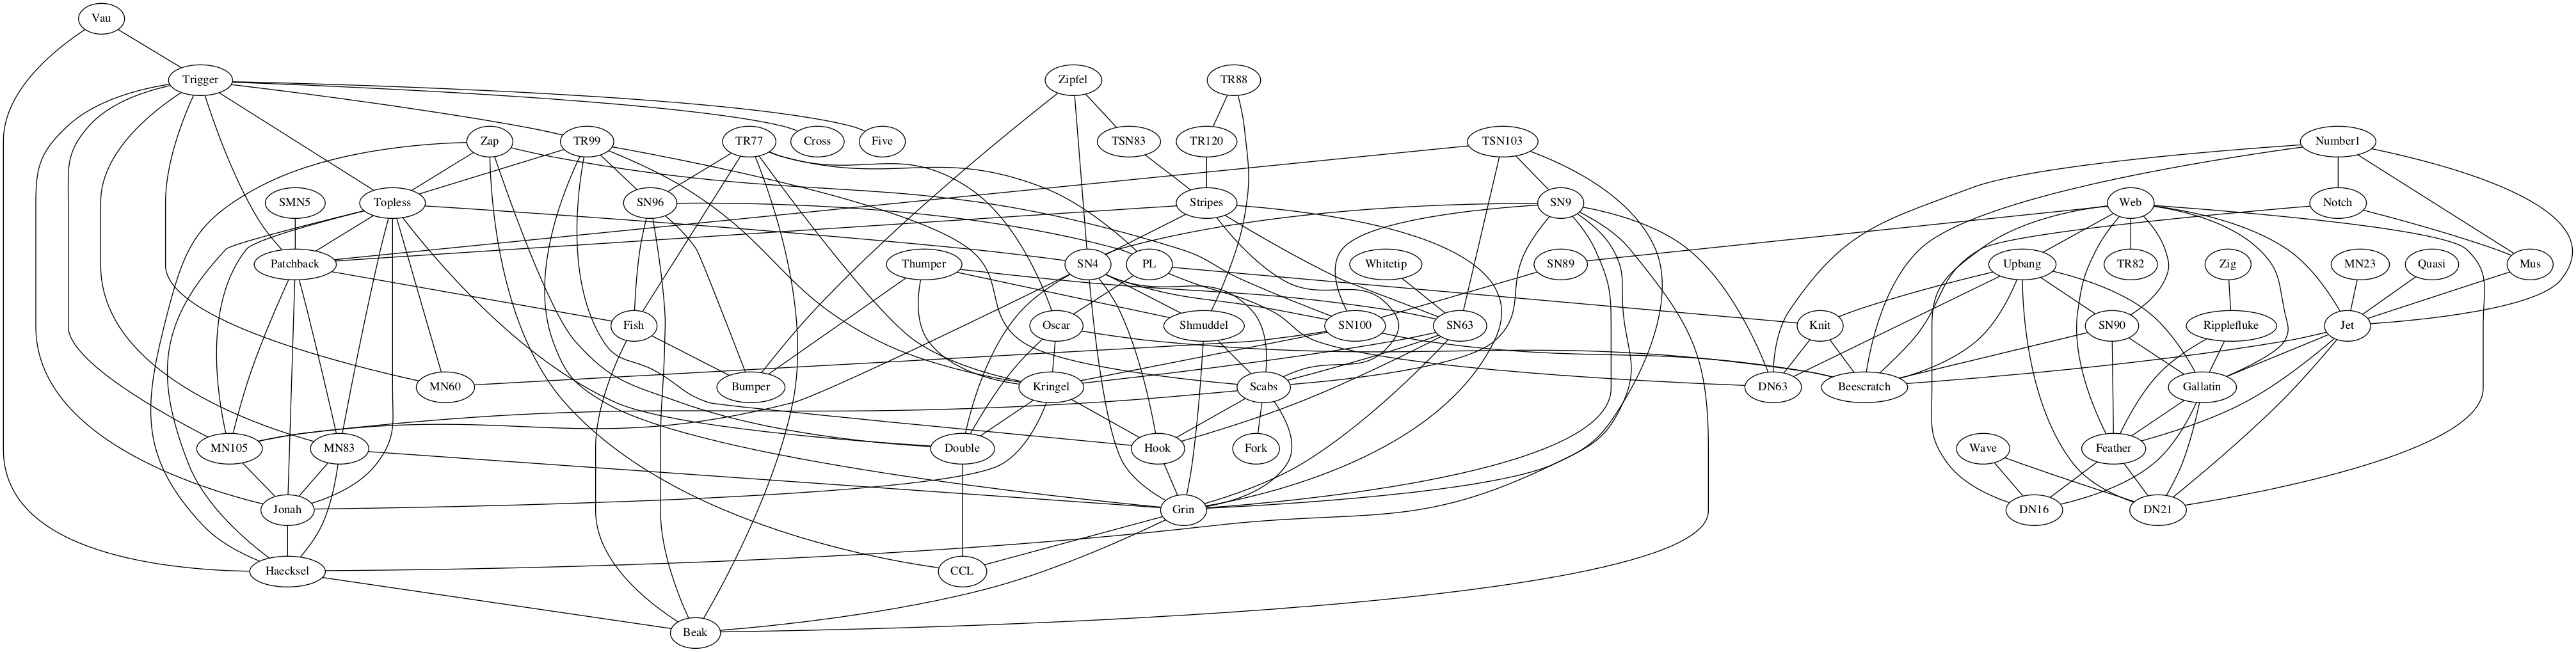
\includegraphics[width=200mm, height=130mm, scale=0.1]{dolphins}
 \end{center}
\newpage
\subsubsection{Test 2}
adjnoun.gml\cite{TESTBENCH21}
\begin{center}
 \includegraphics[width=200mm, height=130mm, scale=0.1]{adjnoun}
 \end{center}
\newpage
\subsubsection{Test 3}
football.gml\cite{TESTBENCH21}
\begin{center}
 \includegraphics[width=200mm, height=130mm, scale=0.1]{football}
 \end{center}
\newpage
\subsubsection{Test 4}
karate.gml\cite{TESTBENCH21}
\begin{center}
 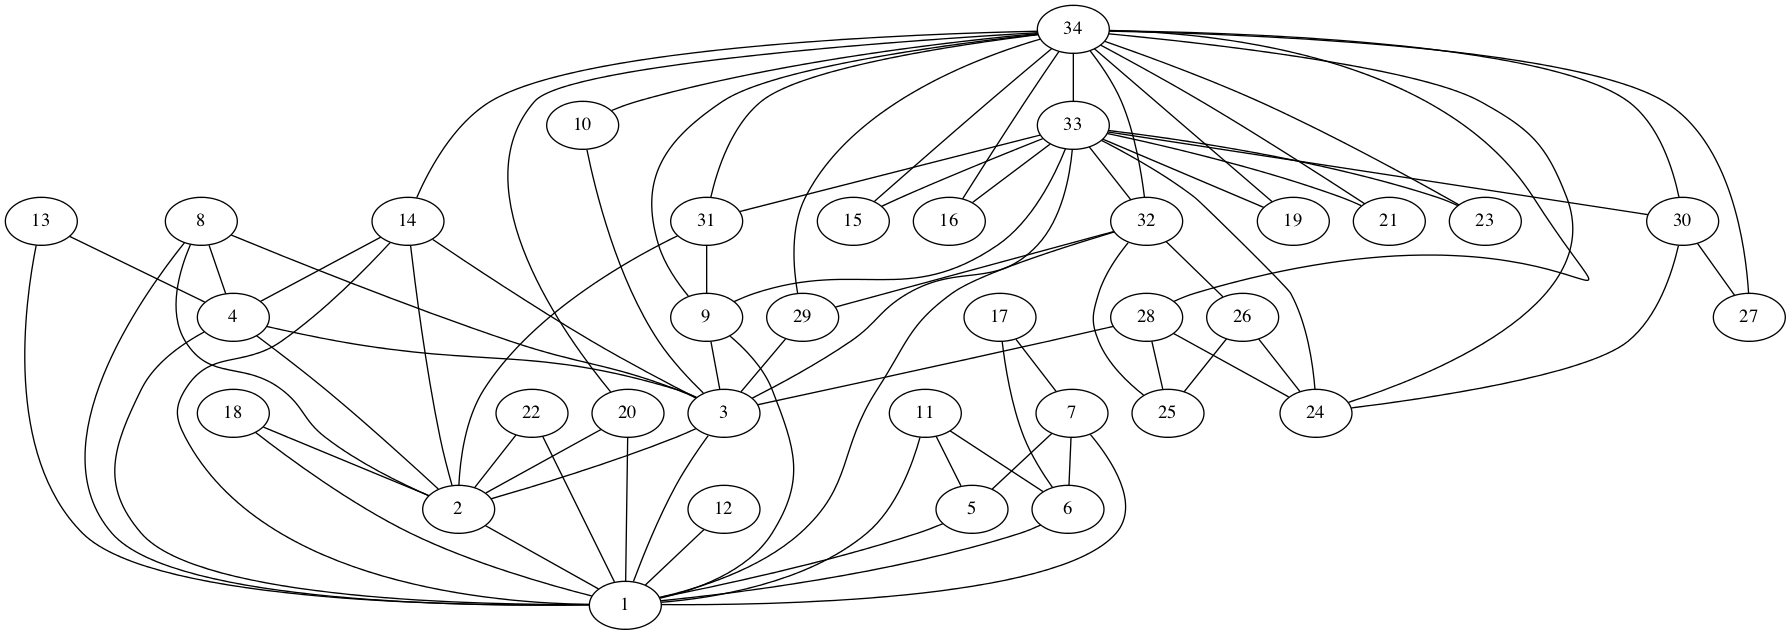
\includegraphics[width=200mm, height=130mm, scale=0.1]{karate}
 \end{center}
\end{landscape}
\nocite{*}
\bibliography{myrefs}
\bibliographystyle{plain}
\end{document}
